\begin{frame}
	\frametitle{Material para armado de estas slides}
    
    \begin{itemize}
	\item Curso de Cyrill Stachniss: \url{https://youtu.be/v-Rm9TUG9LA}

    \item Curso de Cyrill Stachniss (slides): \url{http://ais.informatik.uni-freiburg.de/teaching/ws12/mapping/pdf/slam11-gridmaps-4.pdf}
    \end{itemize}
    

    

\end{frame}

\begin{frame}
    \frametitle{Mapas Grilla de Ocupación (Occupancy Grid Maps)}
    \note{información extraída de https://youtu.be/v-Rm9TUG9LA}
    
    \begin{itemize}
    \item Representación del entorno que usan en general los robots móviles.
    \item Estos tipos de mapas almacenan información sobre que áreas del mapa están ocupados (hay obstáculos) y cuales están libres (se pueden navegar). Se los puede pensar como un ``plano del lugar''.
    \item Permiten realizar planeamiento de caminos.
    \end{itemize}
   
\end{frame}

\begin{frame}
    \frametitle{Motivación: Para qué Mapear}
    \note{información extraída de https://youtu.be/v-Rm9TUG9LA}
    
    \begin{itemize}
        \item Los mapas son requeridos para la mayoría de las tareas de robótica como localización, planeamiento, etc.
        \item Tareas que requieren un entendimiento del entorno (información semántica)
        \item Aprender mapas a partir de mediciones de los sensores es una de las tareas fundamentales de las robótica móvil
    \end{itemize}
    
\end{frame}

\begin{frame}
    \frametitle{Sensores para la creación de mapas}
    \note{información extraída de https://youtu.be/v-Rm9TUG9LA}
    
    \note{Sensores exteroceptivos que nos permiten medir el entorno}
 	
   	\begin{figure}[!h]
    		\centering
    		\subfloat[\scriptsize Cámara]
    		{
    			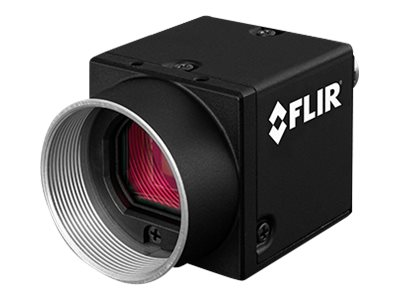
\includegraphics[width=0.15\columnwidth,valign=m]{./images/flir_blackfly_s_camera.jpg}
    		}
    		\subfloat[\scriptsize Cámara Estéreo]
    		{
    			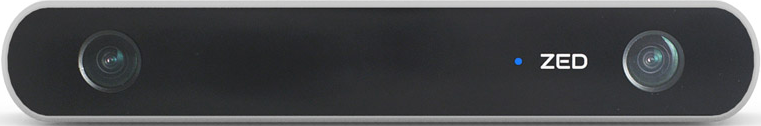
\includegraphics[width=0.2\columnwidth,valign=m]{./images/stereo_camera_zed.png}
    		}
    		\subfloat[\scriptsize Cámara \SI{360}{\degree}]
    		{
    			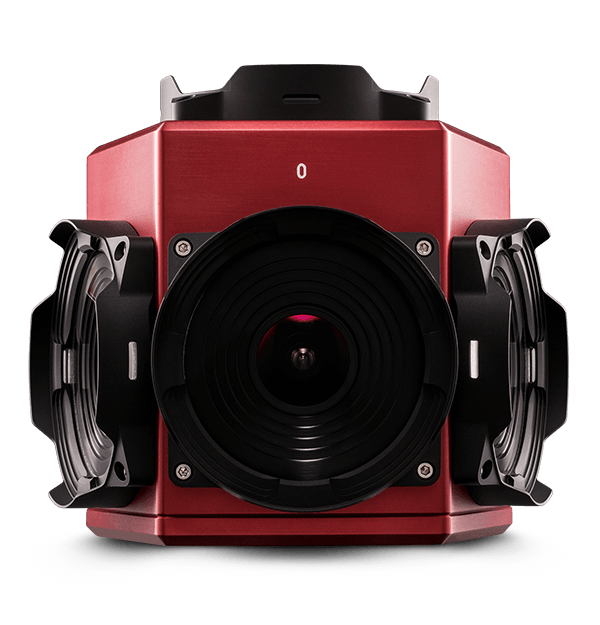
\includegraphics[width=0.1\columnwidth,valign=m]{./images/ladybug5plus_360_camera.png}
    		}
    		\subfloat[\centering \scriptsize Cámara de Luz Estructurada]
    		{
    			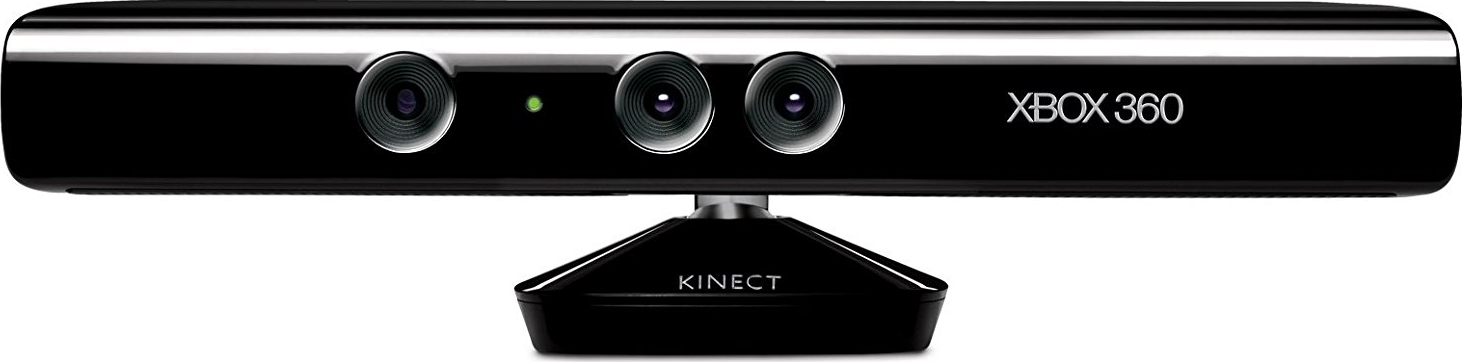
\includegraphics[width=0.2\columnwidth,valign=m]{./images/structured_light_kinect.png}
    		}\\
		   	\subfloat[\scriptsize Cámara ToF]
    		{
    			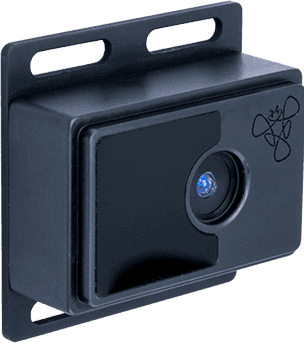
\includegraphics[width=0.15\columnwidth,valign=m]{./images/terabee_time_of_flight_camera.png}
	    	}
    		\subfloat[\scriptsize Cámara de Eventos]
    		{
    			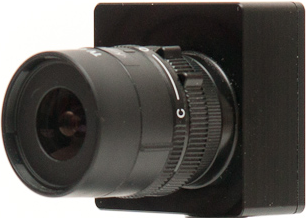
\includegraphics[width=0.2\columnwidth,valign=m]{./images/event_camera_dvs128.png}
    		}
    		\subfloat[\scriptsize LiDAR 2D]
    		{
    			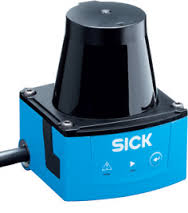
\includegraphics[width=0.15\columnwidth,valign=m]{./images/lidar_sick.jpg}
    		}
	   		\subfloat[\scriptsize LiDAR 3D]
    		{
    			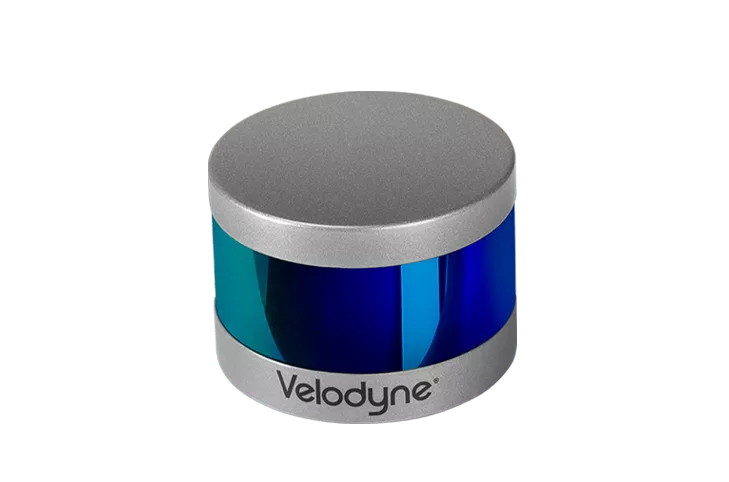
\includegraphics[width=0.15\columnwidth,valign=m]{./images/velodyne_puck.png}
    		}
    	\end{figure}
    
\end{frame}

\begin{frame}
    \frametitle{Mapas Volumétricos vs Features}
    \note{información extraída de https://youtu.be/v-Rm9TUG9LA}
    
    \note{Los feature maps almacen puntos distintivos del entorno}
    
    \note{El feature map correspnode a un trabajo deEduardo Nebot en el victorial park. Los puntos amarillso son los troncos de los árboles.}
    
    \note{El feature map son útiles únicamente para localizarse pero no para navegar por el entorno ya que se desconoce que hay entre los puntos.}
    
    \note{Los mapas volumétricos 2d pueden ser vistos como un plano del piso de la habitación}
    
    \note{Los mapas volumétricos explicitamente representan las áreas libres del entorno.}
    
   	\begin{figure}[!h]
    	\centering
    	\subfloat[Mapa Volumétrico 2D (Grid map)]
    	{
    		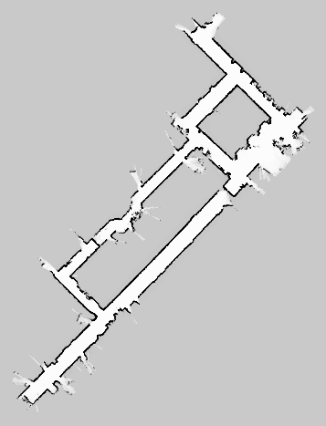
\includegraphics[width=0.23\columnwidth]{./images/volumetric_map_2d.png}
    	}
    	\subfloat[Mapa Volumétrico 3D (Voxel map)]
    	{
    		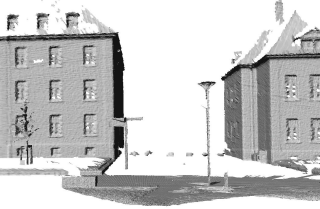
\includegraphics[width=0.3\columnwidth]{./images/volumetric_map_3d.png}
    	}
    	\subfloat[Mapa de features 2D]
    	{
    		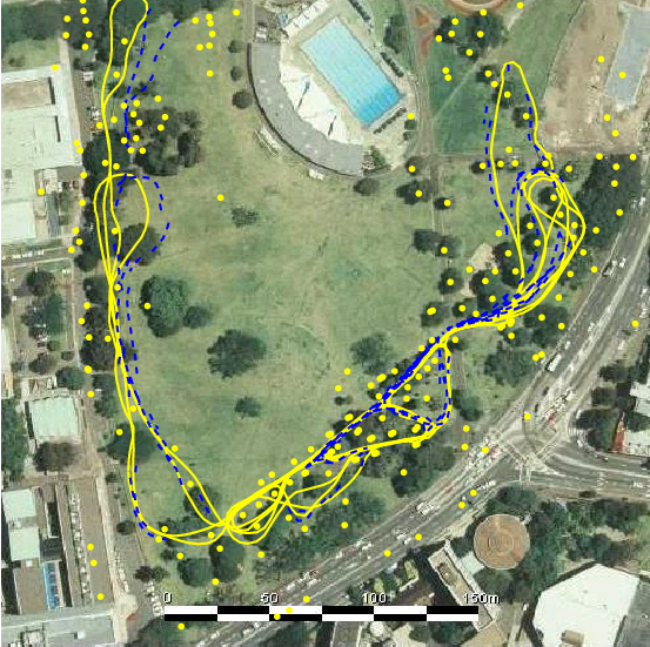
\includegraphics[width=0.3\columnwidth]{./images/feature_map_2d.png}
    	}
    \end{figure}
    
\end{frame}

\begin{frame}
    \frametitle{Quadtree}
    \note{información extraída de https://youtu.be/v-Rm9TUG9LA}
    
    
    \begin{figure}
    	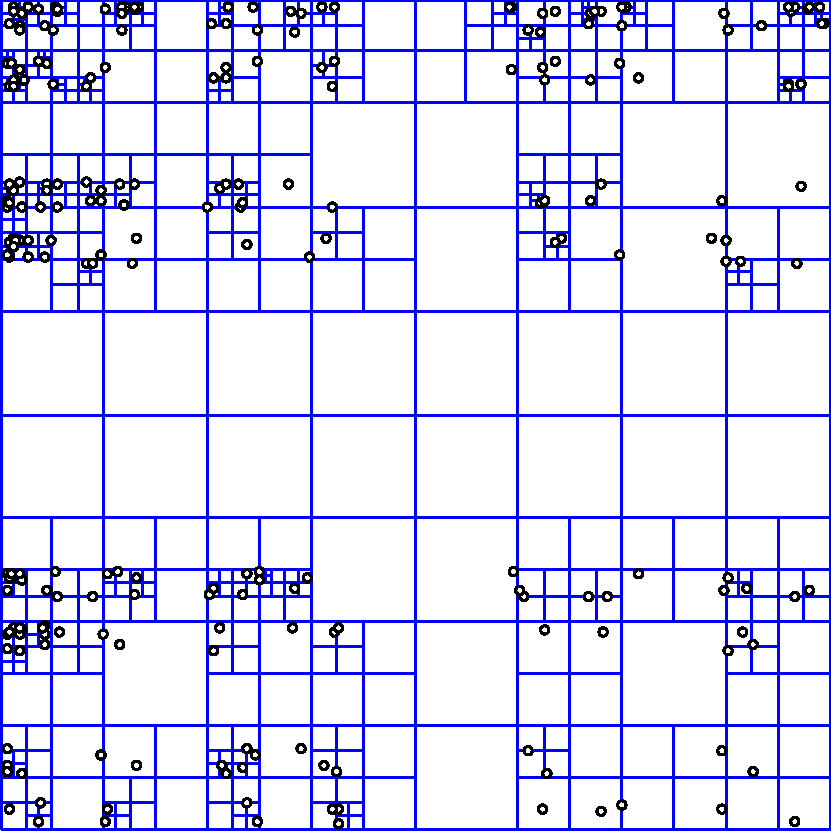
\includegraphics[width=0.5\columnwidth]{./images/quadtree.pdf}
    \end{figure}
    
\end{frame}


\begin{frame}
	\frametitle{Octree (Octomap)}
	\note{información extraída de https://youtu.be/v-Rm9TUG9LA}

	\begin{figure}
		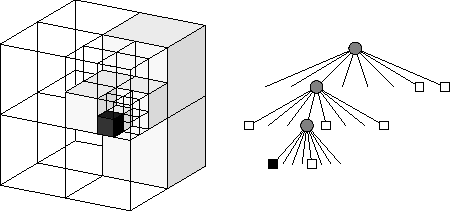
\includegraphics[width=0.5\columnwidth]{./images/octree.pdf}
	\end{figure}
	
	\begin{figure}
		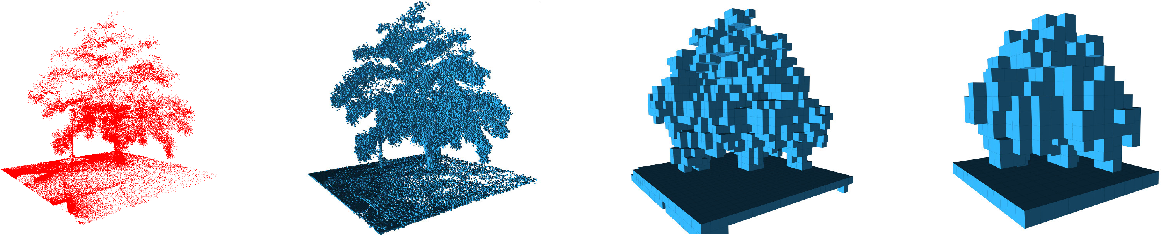
\includegraphics[width=\columnwidth]{./images/octomap.pdf}
	\end{figure}
	
\end{frame}




\begin{frame}
    \frametitle{Mapa de Nube de puntos (Point Cloud Map)}
    \note{información extraída de https://youtu.be/v-Rm9TUG9LA}
    
    
   	\begin{figure}
    	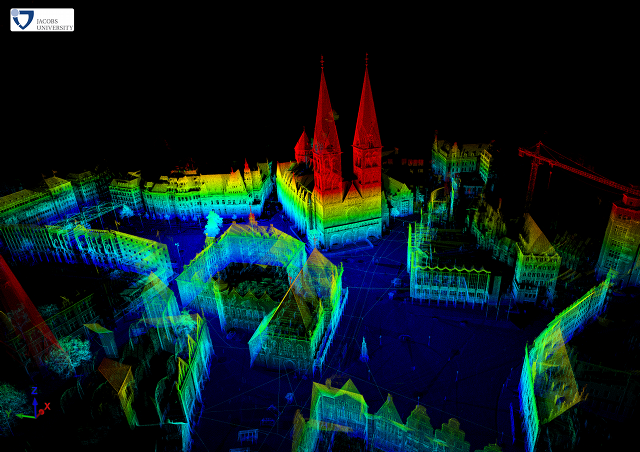
\includegraphics[width=0.6\columnwidth]{./images/point_cloud_map_bremen_city.png}
    \end{figure}
    
\end{frame}

\begin{frame}
    \frametitle{TSDF: Truncated Signed Distance Function}
   
   	\begin{figure}[!h]
	   	\centering
	   	\subfloat[TSDF 2D Function]
	   	{
	   		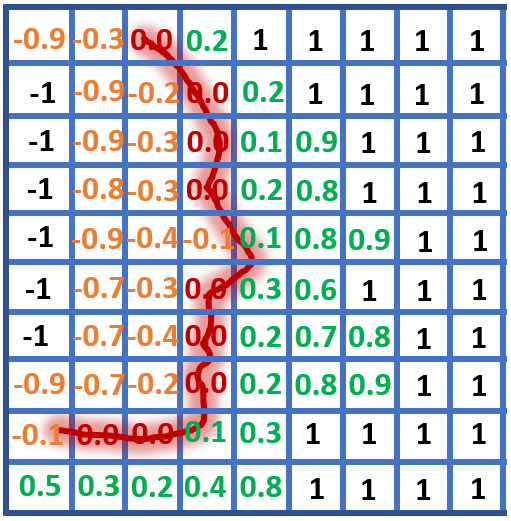
\includegraphics[width=0.45\columnwidth]{./images/tsdf.png}
	   	}
	   	\subfloat[TSDF Reconstruction]
	   	{
	   		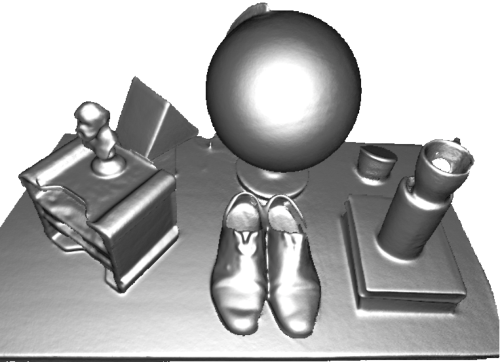
\includegraphics[width=0.45\columnwidth]{./images/tsdf_reconstruction.pdf}
	   	}
   \end{figure}
    
\end{frame}


\begin{frame}
	\frametitle{Mapa Semántico (Semantic Map)}
	\note{información extraída de https://youtu.be/v-Rm9TUG9LA}
	
   	\begin{figure}
    	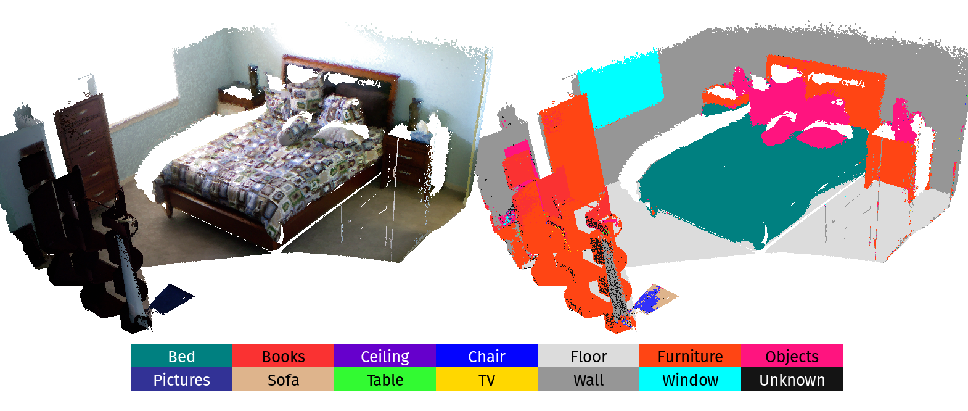
\includegraphics[width=0.8\columnwidth]{./images/semantic_map_semanticfusion.png}
	\end{figure}
	
\end{frame}


\begin{frame}
	\frametitle{Mapa Topológico}
	\note{información extraída de https://youtu.be/v-Rm9TUG9LA}
	
	\begin{figure}
		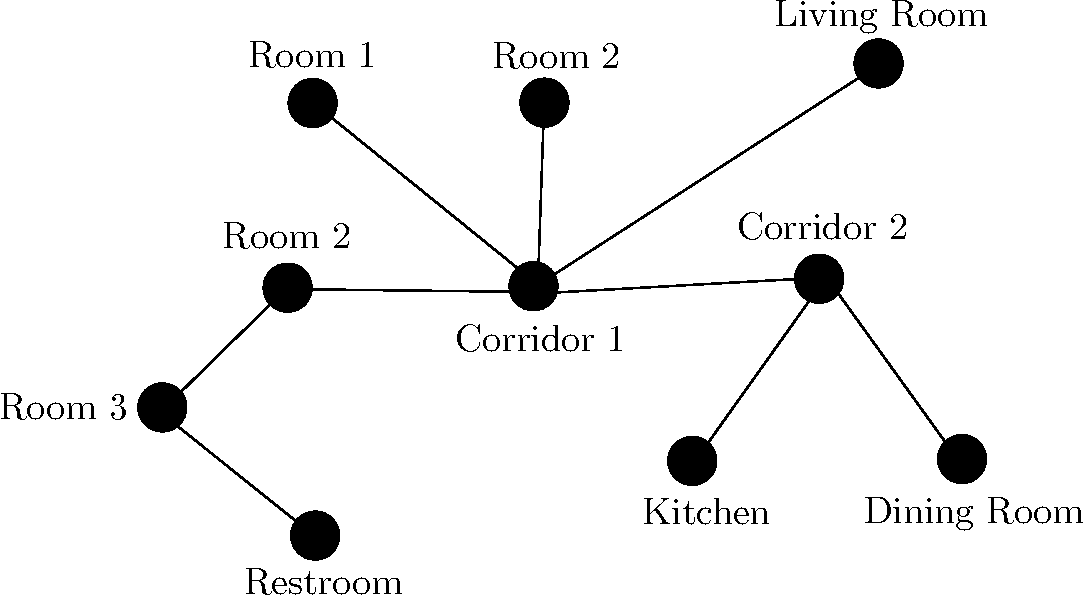
\includegraphics[width=0.8\columnwidth]{./images/topological_map.pdf}
	\end{figure}
	
\end{frame}

\begin{frame}
    \frametitle{Recontrucción de mapas}
    \note{información extraída de https://youtu.be/v-Rm9TUG9LA}
    
    \begin{itemize}
        \item Computar el mapa más probable dado las mediciones de los sensores
        \begin{equation*}
            \map^{*} = \argmax p(\map | \controlCommand_{1}, \observation_{1}, \dots, \controlCommand_{t}, \observation_{t})
        \end{equation*}
        \item Sin embargo, vamos a abordar un problema más simple: veamos cómo computar el mapa dada la pose del robot (la localización resuelta) y las mediciones de los sensores.
        \begin{equation*}
            \map^{*} = \argmax p(\map | \state_{1}, \observation_{1}, \dots, \state_{t}, \observation_{t})
        \end{equation*}
    \end{itemize}

    \alert{Resolver la localización y el mapeo al mismo tiempo es resolver el problema de SLAM, y lo veremos más adelante.}
    
\end{frame}

\begin{frame}
    \frametitle{Grid Maps}
    \note{información extraída de https://youtu.be/v-Rm9TUG9LA}
    
    \note{}
    
    \begin{itemize}
        \item Modelos de mapa de ocupación del espacio
        \item Discretiza el mundo en celdas
        \item La estructura de la grilla está fija (el tamaño de las celdas y la grilla es fijo)
        \item Cada celda puede estar ocupada o libre
        \item Modelo no-paramétrico (es decir, una celda no está parametrizada como una gaussiana por ejemplo sino que está libre u ocupada)
        \item El tamaño de los mapas de grilla puede requerir mucha memoria (en el caso 3D sobre todo)
        \item No requiere de un detector de features específico (sino que utilizamos las mediciones crudas del sensor)
    \end{itemize}
\end{frame}

\begin{frame}
    \frametitle{Ejemplo de Mapa de Grilla de Ocupación}
    \note{información extraída de https://youtu.be/v-Rm9TUG9LA}
    
    Podemos representar a un \emph{Occupancy Grid Map} con una imagen donde un píxel es blanco si está libre y negro si está ocupado (hay algún objeto). Un píxel gris representa un espacio que no conocemos.
    
  	\begin{figure}[!h]
    		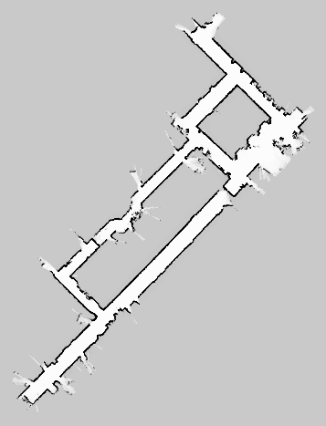
\includegraphics[width=0.23\columnwidth]{./images/volumetric_map_2d.png}
    \end{figure}


	Los \emph{Occupancy Grid Maps} hacen suposiciones acerca del mundo.
       
\end{frame}

\begin{frame}
    \frametitle{Suposiciones de Occupancy Grid Maps}
    \note{información extraída de https://youtu.be/v-Rm9TUG9LA}
    
    \begin{block}{Suposición 1}
	    El área de una celda esta o completamente libre u ocupada.
    \end{block}

	Esta suposición no sucede en la realidad ya que puede haber objetos que sean menores que el tamaño de la celda u objetos que cubran parcialmente una celda.
	
  	\begin{figure}[!h]
		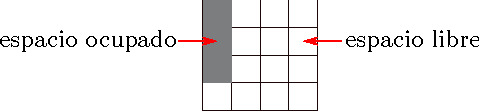
\includegraphics[width=0.7\columnwidth]{./images/grid_map.pdf}
	\end{figure}
	
\end{frame}

\begin{frame}
	\frametitle{Representación: Probabilidad de Ocupación}
	\note{información extraída de https://youtu.be/v-Rm9TUG9LA}

	\begin{itemize}
	\item Cada celda es una {\bf variable aleatoria binaria} que modela la ocupación de la celda.
	\item La celda está ocupada: $p(\map_{i}) = 1$
	\item La celda está libre: $p(\map_{i}) = 0$
	\item No tenemos información: $p(\map_{i}) = 0.5$
	\end{itemize}
	
	\begin{figure}[!h]
		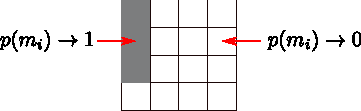
\includegraphics[width=0.7\columnwidth]{./images/grid_map_representation.pdf}
	\end{figure}
\end{frame}

\begin{frame}
    \frametitle{Probabilidad de Ocupación}
    \note{información extraída de https://youtu.be/v-Rm9TUG9LA}
   	\begin{itemize}
    	\item Cada celda es una {\bf variable aleatoria binaria} que modela la ocupación de la celda.
    	\item Notación:
   	   	\begin{itemize}
    		\item La probabilidad de que la celta este ocupada, la notamos:\\ $P(\mapRandomVariable_{i} = occ) = P_{occ}(\mapRandomVariable_{i}) = p(\map_{i})$
    		\item La probabilidad de que la celta este libre, la notamos:\\ $P(\mapRandomVariable_{i} = free) = P_{free}(\mapRandomVariable_{i}) = 1 - P_{occ}(\mapRandomVariable{i}) = p(\neg \map_{i})$
    	\end{itemize}
    \end{itemize}
    
\end{frame}

\begin{frame}
    \frametitle{Suposición 2}
    \note{información extraída de https://youtu.be/v-Rm9TUG9LA}
    El mundo es estático.
    
     	\begin{figure}[!h]
    	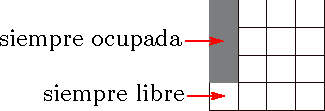
\includegraphics[width=0.7\columnwidth]{./images/grid_map_static_assumption.pdf}
    \end{figure}
    
    Esto no es cierto en la práctica ya que hay objetos que se mueven por el entorno o el entorno es modificado (personas caminando, objetos que se mueven de un lugar a otro, etc).
    
\end{frame}

\begin{frame}
	\frametitle{Suposición 3}
	\note{información extraída de https://youtu.be/v-Rm9TUG9LA}
	Las celdas (las variables aleatorias) son independientes entre sí.
	
	\begin{figure}[!h]
		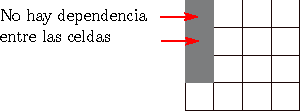
\includegraphics[width=0.7\columnwidth]{./images/grid_map_independency_assumption.pdf}
	\end{figure}
	
	Nuevamente esto no es cierto en el la práctica, pero asumimos esta independencia para simplificar el modelo.
	
\end{frame}

\begin{frame}
    \frametitle{Distribución conjunta}
    \note{información extraída de https://youtu.be/v-Rm9TUG9LA}
    
    Un mapa de ocupación entonces es la distribución de probabilidad representando todo el mapa del entorno. La distribución de probabilidad de todo el mapa es la probabilidad conjunta (\emph{joint belief}) del valor de todas las celdas individuales.
    
   	\begin{figure}[!h]
    	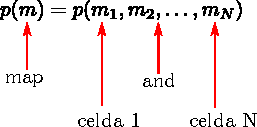
\includegraphics[width=0.5\columnwidth]{./images/joint_distribution.pdf}
    \end{figure}
    
\end{frame}

\begin{frame}
    \frametitle{Representación}
    \note{información extraída de https://youtu.be/v-Rm9TUG9LA}
    La distribución de probabilidad del mapa esta dada por el producto de las celdas.
    
   	\begin{figure}[!h]
    	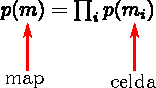
\includegraphics[width=0.3\columnwidth]{./images/map_probability_distribution.pdf}
    \end{figure}
    
\end{frame}

\begin{frame}
	\frametitle{Estimando un Mapa por medio de mediciones}
	\note{información extraída de https://youtu.be/v-Rm9TUG9LA}
	
	Dadas las mediciones $\observation_{i:t}$ y las poses $\state_{1:t}$ del sensor, estimamos el mapa como
	
   	\begin{figure}[!h]
    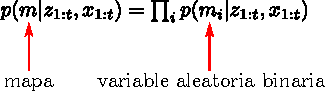
\includegraphics[width=0.3\columnwidth]{./images/map_from_sensor_data.pdf}
    \end{figure}

    En este caso, utilizaremos sensores de rango, pero necesitamos un sensor que nos diga si una celda está ocupada o libre.
	
	
	Podemos utilizar un {\bf Filtro de Bayes Binario} para estimar la probabilidad de las variables aleatorias binarias. Asumimos un estado (mapa) estático, no cambia en el tiempo. Una celda ocupada/libre permanecera por siempre ocupada/libre.
	
\end{frame}

\begin{frame}
	\frametitle{Filtro de Bayes Binario para Estado Estático}
	\note{información extraída de https://youtu.be/v-Rm9TUG9LA}
    
    \TODO{colorear los resultados de los términos que cambian}
	
	\begin{align*}
		\only<1->{
			p(\map_{i}| \observation_{1:t}, \state_{1:t}) \overset{\text{Regla de Bayes}}{=}& \dfrac{p(\observation_{t} | \map_{i}, \observation_{1:t-1}, \state_{1:t}) p(\map_{i} | \observation_{1:t-1}, \state_{1:t})}{p(\observation_{t} | \observation_{1:t-1}, \state_{1:t})}}
		\\
		\only<2->{
			\overset{\text{Markov}}{=}& \dfrac{p(\observation_{t} | \map_{i}, \state_{1:t}) p(\map_{i} | \observation_{1:t-1}, \state_{1:t-1})}{p(\observation_{t} | \observation_{1:t-1}, \state_{1:t})}}
		\\
		\only<3->{
		\overset{\text{Regla de Bayes}}{=}& \dfrac{p(\map_{i} | \observation_{t}, \state_{t}) p(\observation_{t} | \state_{t}) p(\map_{i} | \observation_{1:t-1}, \state_{1:t-1})}{p(\map_{i} | \state_{t})p(\observation_{t} | \observation_{1:t-1}, \state_{1:t})}}
		\\
		\only<4->{
		\overset{\text{independencia}}{=}& \dfrac{p(\map_{i} | \observation_{t}, \state_{t}) p(\observation_{t} | \state_{t}) p(\map_{i} | \observation_{1:t-1}, \state_{1:t-1})}{p(\map_{i})p(\observation_{t} | \observation_{1:t-1}, \state_{1:t})}}
	\end{align*}

	\only<2>{Aplicamos Markov: La observación de ahora es independiente de las mediciones y poses anteriores. También, en el segundo término podemos ignorar $x_{t}$. Esto es, saber mi posición en el instante $t$ sin tener mediciones en dicho instante, no me va a servir de determinar si una celda esta libre u ocupada. El único caso dónde esto puede servir en la práctica es si el robot se encuentra encima de esa celda, y por tanto la celda esta libre de obstáculos ya que está parada sobre ella.}
	
	\only<3>{Aplicamos Regla de Bayes en el primer término de la multiplicación}
	
	\only<4>{Asumimos Independencia: nuevamente saber donde estamos no nos sirve para saber si una celda está libre u ocupada.}
	
	\only<5>{Como estamos con una variable aleatoria binaria entonces podemos hacer la misma derivación para el caso en que la celda este vacía
	
	\begin{equation*}
		p(\neg \map_{i}| \observation_{1:t}, \state_{1:t}) \overset{\text{Regla de Bayes}}{=} \dfrac{p(\neg \map_{i} | \observation_{t}, \state_{t}) p(\observation_{t} | \state_{t}) p(\neg \map_{i} | \observation_{1:t-1}, \state_{1:t-1})}{p(\neg \map_{i})p(\observation_{t} | \observation_{1:t-1}, \state_{1:t})}
	\end{equation*}
	}
\end{frame}


\begin{frame}
	\frametitle{Filtro de Bayes Binario para Estado Estático}
	\note{información extraída de https://youtu.be/v-Rm9TUG9LA}
	
	Hagamos un truco matemático...\\
    Podemos computar el ratio de ambas probabilidades obteniendo:
	
    \only<1>{
	\begin{equation*}
		\dfrac{p(\map_{i}| \observation_{1:t}, \state_{1:t})}{p(\neg \map_{i}| \observation_{1:t}, \state_{1:t})} = \dfrac{\dfrac{p(\map_{i} | \observation_{t}, \state_{t}) p(\observation_{t} | \state_{t}) p(\map_{i} | \observation_{1:t-1}, \state_{1:t-1})}{p(\map_{i})p(\observation_{t} | \observation_{1:t-1}, \state_{1:t})}} {\dfrac{p(\neg \map_{i} | \observation_{t}, \state_{t}) p(\observation_{t} | \state_{t}) p(\neg \map_{i} | \observation_{1:t-1}, \state_{1:t-1})}{p(\neg \map_{i})p(\observation_{t} | \observation_{1:t-1}, \state_{1:t})}}
	\end{equation*}
    }

    \only<2>{
	\begin{equation*}
	\dfrac{p(\map_{i}| \observation_{1:t}, \state_{1:t})}{p(\neg \map_{i}| \observation_{1:t}, \state_{1:t})} = \dfrac{\dfrac{p(\map_{i} | \observation_{t}, \state_{t}) \cancel{p(\observation_{t} | \state_{t})} p(\map_{i} | \observation_{1:t-1}, \state_{1:t-1})}{p(\map_{i})\cancel{p(\observation_{t} | \observation_{1:t-1}, \state_{1:t})}}} {\dfrac{p(\neg \map_{i} | \observation_{t}, \state_{t}) \cancel{p(\observation_{t} | \state_{t})} p(\neg \map_{i} | \observation_{1:t-1}, \state_{1:t-1})}{p(\neg \map_{i})\cancel{p(\observation_{t} | \observation_{1:t-1}, \state_{1:t})}}}
	\end{equation*}
    }

    \only<3>{
    \begin{equation*}
        \dfrac{p(\map_{i}| \observation_{1:t}, \state_{1:t})}{p(\neg \map_{i}| \observation_{1:t}, \state_{1:t})} = \dfrac{\dfrac{p(\map_{i} | \observation_{t}, \state_{t}) p(\map_{i} | \observation_{1:t-1}, \state_{1:t-1})}{p(\map_{i})}} {\dfrac{p(\neg \map_{i} | \observation_{t}, \state_{t}) p(\neg \map_{i} | \observation_{1:t-1}, \state_{1:t-1})}{p(\neg \map_{i})}}
    \end{equation*}
    }

    \only<4->{
    \begin{align*}
        \dfrac{p(\map_{i}| \observation_{1:t}, \state_{1:t})}{p(\neg \map_{i}| \observation_{1:t}, \state_{1:t})} 
        =& \dfrac{p(\map_{i} | \observation_{t}, \state_{t}) p(\map_{i} | \observation_{1:t-1}, \state_{1:t-1} p(\neg \map_{i})} {p(\neg \map_{i} | \observation_{t}, \state_{t}) p(\neg \map_{i} | \observation_{1:t-1}, \state_{1:t-1})p(\map_{i})}\\
    \only<5>{
        =& \dfrac{p(\map_{i} | \observation_{t}, \state_{t})}{1 - p(\map_{i} | \observation_{t}, \state_{t})}
        %
        \dfrac{p(\map_{i} | \observation_{1:t-1}, \state_{1:t-1})}{1- p(\map_{i} | \observation_{1:t-1}, \state_{1:t-1})}
        %
        \dfrac{1 - p(\map_{i})} {p(\map_{i})}
    }
    \only<6>{
        =& \underbrace{\dfrac{p(\map_{i} | \observation_{t}, \state_{t})}{1 - p(\map_{i} | \observation_{t}, \state_{t})}}_{\text{usa } \observation_{t}}
        %
        \underbrace{\dfrac{p(\map_{i} | \observation_{1:t-1}, \state_{1:t-1})}{1- p(\map_{i} | \observation_{1:t-1}, \state_{1:t-1})}}_{\text{término recursivo}}
        %
        \underbrace{\dfrac{1 - p(\map_{i})} {p(\map_{i})}}_{\text{prior}}
    }
    \end{align*}
    }

    \only<5>{Reescribimos y Reagrupamos términos}
    \only<6>{El primer término utiliza información actual.\\
             El segundo término utiliza información del pasado.\\
             El tercer término es un prior (información que asumimos del mapa)
    }
\end{frame}


\begin{frame}
    \frametitle{Del ratio a la probabilidad}
    \note{información extraída de https://youtu.be/v-Rm9TUG9LA}

    Podemos transformar fácilmente este ratio denominado \emph{odds ratio} (razón de probabilidades) en una probabilidad:
    
    \begin{align*}
        Odds(x) &= \dfrac{p(x)}{1-p(x)}\\
        p(x) &= Odds(x) - Odds(x) p(x)\\
        p(x)(1 + Odds(x)) &= Odds(x)\\
        p(x) &= \dfrac{Odds(x)}{1 + Odds(x)}\\
        p(x) &= \dfrac{1}{1 + \dfrac{1}{Odds(x)}}
    \end{align*}

    De esta manera podemos convertir odds a probabilidades y de probabilidades a odds.    
    
\end{frame}


\begin{frame}
    \frametitle{Del ratio a la probabilidad}
    \note{información extraída de https://youtu.be/v-Rm9TUG9LA}
    
    Utilizando $p(x) = \dfrac{1}{1 + \dfrac{1}{Odds(x)}}$ en el odds ratio que habíamos encontrado
    
    \begin{equation*}
         \dfrac{p(\map_{i}| \observation_{1:t}, \state_{1:t})}{p(\neg \map_{i}| \observation_{1:t}, \state_{1:t})} = \dfrac{p(\map_{i} | \observation_{t}, \state_{t})}{1 - p(\map_{i} | \observation_{t}, \state_{t})}
        %
        \dfrac{p(\map_{i} | \observation_{1:t-1}, \state_{1:t-1})}{1- p(\map_{i} | \observation_{1:t-1}, \state_{1:t-1})}
        %
        \dfrac{1 - p(\map_{i})} {p(\map_{i})}
    \end{equation*}

tenemos entonces:

    \begin{equation*}
    p(\map_{i}| \observation_{1:t}, \state_{1:t}) =
    \left[
        1 + 
         \dfrac{1 - p(\map_{i} | \observation_{t}, \state_{t})}{p(\map_{i} | \observation_{t}, \state_{t})}
        %
        \dfrac{1- p(\map_{i} | \observation_{1:t-1}, \state_{1:t-1})}{p(\map_{i} | \observation_{1:t-1}, \state_{1:t-1})}
        %
        \dfrac{p(\map_{i})}{1 - p(\map_{i})}
    \right]^{-1}
    \end{equation*}

    Por razones de eficiencia, se realizan los cálculos aplicando el logaritmo al ratio de las probabilidades (notación \emph{log odds}).
\end{frame}

\begin{frame}
    \frametitle{Notación log-odds}
    \note{información extraída de https://youtu.be/v-Rm9TUG9LA}
    \begin{equation*}
        \dfrac{p(\map_{i}| \observation_{1:t}, \state_{1:t})}{1 - p(\map_{i}| \observation_{1:t}, \state_{1:t})} =  \underbrace{\dfrac{p(\map_{i} | \observation_{t}, \state_{t})}{1 - p(\map_{i} | \observation_{t}, \state_{t})}}_{\text{usa } \observation_{t}}
        %
        \underbrace{\dfrac{p(\map_{i} | \observation_{1:t-1}, \state_{1:t-1})}{1- p(\map_{i} | \observation_{1:t-1}, \state_{1:t-1})}}_{\text{término recursivo}}
        %
        \underbrace{\dfrac{1 - p(\map_{i})} {p(\map_{i})}}_{\text{prior}}
    \end{equation*}

    \begin{equation*}
   l(\map_{i}| \observation_{1:t}, \state_{1:t}) =  \log \left( \dfrac{p(\map_{i} | \observation_{1:t}, \state_{1:t})}{1 - p(\map_{i} | \observation_{1:t}, \state_{1:t})} \right)
    \end{equation*}

    Aplicando un logaritmo a ambos lados entonces, en el lado derecho de la igualdad se convierten las multiplicaciones en sumas. haciendo que el algoritmo sea rápido ya que solo tenemos que aplicar tres sumas.

\end{frame}

\begin{frame}
    \frametitle{Notación log-odds}
    \note{información extraída de https://youtu.be/v-Rm9TUG9LA}

    \begin{itemize}
        \item Log odds ratio está definido por:
        \begin{equation*}
            l(x) = \log \dfrac{p(x)}{1-p(x)}
        \end{equation*}
        \item podemos de despejar $p(x)$
        \begin{equation*}
            p(x) = 1 - \dfrac{1}{1 + \exp l(x)}
        \end{equation*}
    \end{itemize}
    
\end{frame}

\begin{frame}
    \frametitle{Mapeo de ocupación utilizando Log Odds}
    \note{información extraída de https://youtu.be/v-Rm9TUG9LA}
    
    \begin{itemize}
        \item Log odds ratio está definido por:
        \begin{equation*}
            l(\map_{i}| \observation_{1:t}, \state_{1:t}) = \underbrace{l(\map_{i}| \observation_{t}, \state_{t})}_{\text{inverse sensor model}} + \underbrace{l(\map_{i}| \observation_{1:t-1}, \state_{1:t-1})}_{\text{término recursivo}} - \underbrace{l(\map_{i})}_{\text{prior}}
        \end{equation*}
        \item reescribiendo:
        \begin{equation*}
            l_{t,i} = inv\_sensor\_model(\map_{i}, \state_{t}, \observation_{t}) + l_{t-1,i} - l_{0}
        \end{equation*}
    \end{itemize}
    
    Entonces, el valor de la celda $i$ en el instante $t$ se actualiza con la suma del $inv\_sensor\_model$ (término que depende de mi observación actual) y el valor anterior que tenía la celda $i$, menos el prior de información.
    
\end{frame}

\begin{frame}
	\frametitle{Forward measurement model vs inverse measurement model}
	\note{información extraída de https://youtu.be/v-Rm9TUG9LA}
    
    \TODO{explicar mejor invese sensor model y formard sensor model}
   
	El algoritmo \emph{occupancy grid mapping} requiere un modelo marginalized inverse measurement model, $p(\map_{i}|\state, \observation )$. Esta probabilidad se llama inversa ya que razona de efectos a causas: proporciona información sobre el mundo condicionada a una medida provocada por este mundo.

	Los \emph{inverse models} se utilizan a menudo en situaciones en las que las medidas son más complejas que el estado binario. Un ejemplo de tal situación es el problema de estimar si una puerta está cerrada o no a partir de imágenes de una cámara. Aquí el estado es extremadamente simple, pero el espacio de todas las mediciones es enorme. Es más fácil entonces idear una función que calcule la probabilidad de que una puerta este cerrada a partir de una imagen, que describir la distribución de probabilidad sobre todas las imágenes que muestran una puerta cerrada. En otras palabras, es más fácil implementar un modelo de sensor inverso que uno directo.
	
	
	forward measurement model vs inverse measurement model
	\url{https://www.cs.cmu.edu/~thrun/papers/thrun.occ-journal.pdf}
	\url{http://robots.stanford.edu/papers/thrun.iros01-occmap.pdf}
	
	Los forward models describen la física del entorno, desde las causas (ocupación) hasta los efectos (medidas). Son denotados $p(\observation | \map)$.
	
\end{frame}

\begin{frame}
    \frametitle{Algoritmo de Mapeo de Ocupación}
    \note{información extraída de https://youtu.be/v-Rm9TUG9LA}
    
   \begin{algorithmic}[1]
       \State occupancy\_grid\_mapping($\left\lbrace l_{t-1,i} \right\rbrace, \state_{t}, \observation_{t}$)
       \For todas las celdas $\map_{i}$
       \If{$\map_{i}$ está siendo observada por $\observation_{t}$}
            \State $l_{t,i} = inv\_sensor\_model(\map_{i}, \state_{t}, \observation_{t}) + l_{t-1,i} - l_{0}$
       \Else
       \State $l_{t,i} = l_{t-1,i}$
       \EndIf
       \EndFor
       
       \State \Return $\left\lbrace l_{t,i} \right\rbrace$
   \end{algorithmic}
    Muy eficente, ya que solo tenemos que hacer sumas!
\note{Moravec and Elfes propusieron occupancy grid mapping en los 80's. Desarrollado para sensores sonares ruidosos. También llamado Mapping with known poses}

\end{frame}

\begin{frame}
    \frametitle{Inverse sensor model para Laser Range Finder}
    \note{información extraída de https://youtu.be/v-Rm9TUG9LA}
    
   	\begin{figure}[!h]
        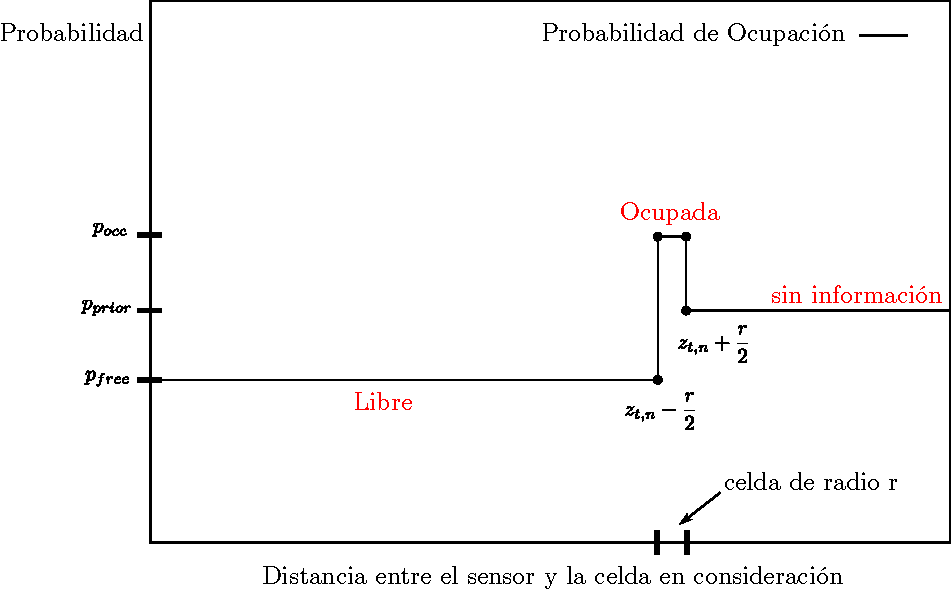
\includegraphics[width=0.8\columnwidth]{./images/inverse_senor_model_range_finder.pdf}
    \end{figure}
    
\end{frame}

\begin{frame}
    \frametitle{Bresenham's line algorithm}
    \note{información extraída de https://youtu.be/v-Rm9TUG9LA}
    
    
    \TODO{agregar imagen de Bresenham's line algorithm como hace cyrill stachniss}
\end{frame}

\begin{frame}
    \frametitle{Agregar vídeo de ejemplo}
    \note{información extraída de https://youtu.be/v-Rm9TUG9LA}
   
    
    \TODO{agregar vídeo de ejemplo de grid mapping como hace cyrill stachniss}
\end{frame}

\begin{frame}
    \frametitle{Resumen: Occupancy Grid Map}
    \note{información extraída de https://youtu.be/v-Rm9TUG9LA}
    
    \TODO{agregar resumen de Occupancy Grid Map como hace cyrill stachniss}
\end{frame}

